\chapter{Deep Learning for Text Classification}

FFN structure has problems when dealing with text representations:
\begin{itemize}
	\item Texts are composed of discrete objects (words, characters), FFN expect
numerical inputs
	\item Texts lenghts are variable, input size of a FFN is fixed
\end{itemize}
Possible solutions:
\begin{itemize}
	\item Word embeddings to convert text sequences into numerical data
	\item Recurrent networks or other alternatives to process sequences
\end{itemize}
These problems appear in other objects: speech, handwritten text, general
temporal sequences, protein chains, video, large images,\dots

\section{Word Embeddings}

\begin{paracol}{2}
   
   Discrete symbols can be encoded by assigning them one or more numbers
   E.g., ``a'' $\rightarrow 1$, ``b'' $\rightarrow 2$, \dots
   
   To fit the natural input of neural networks, many representations are possible:
   \begin{itemize}
      \item One-hot encoding (or local) - a binary vector, size of vocabulary, 1 in the position of the symbol, 0 in the rest of positions
      \item Distributed - binary encoding of an assigned natural number
      \item Embedding - real values vector of a predefined dimension D
   \end{itemize}
      
   \switchcolumn

   \begin{figure}[htbp]
      \centering
      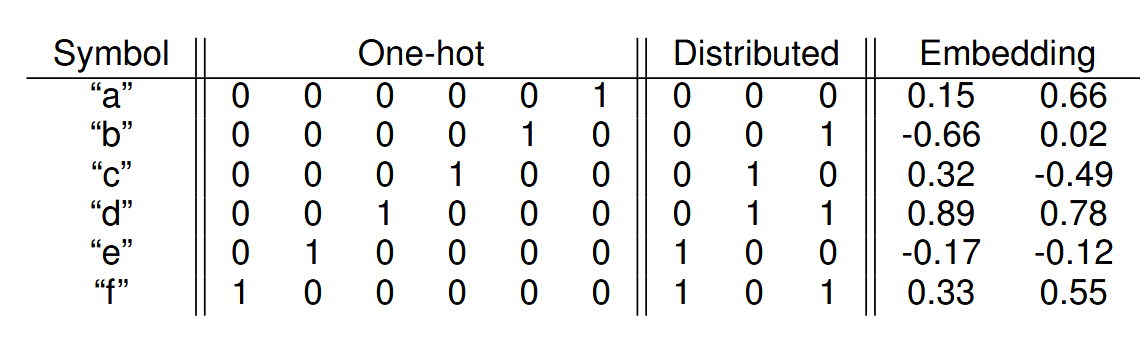
\includegraphics{images/09/embeddings.png}
      \caption{Word Embeddings}
      \label{fig:09/embeddings}
   \end{figure}

\end{paracol}